\chapter{Vectorized Backtesting}


Backtesting is the process of testing a trading strategy using historical data, allowing traders to evaluate and refine their strategies before implementing them in live markets.
In this project, the implemented backtester provides vectorized backtesting for both technical indicator-based strategies and machine learning-based strategies.
Vectorization, a form of array programming, allows operations typically done on scalars to be extended to multidimensional arrays.
In Python's data ecosystem, \textit{pandas}, with its \textit{DataFrame} class, deeply integrates with \textit{NumPy}, benefiting from its vectorization principles.
It facilitates compact code, faster execution compared to conventional Python loops, and efficient handling of time series data. This is particularly useful in financial algorithm implementations, especially vectorized backtesting.

\section{Input Data}


All the data used in this project is downloaded using the \texttt{data\_retriever} module, which establishes a connection with the Binance server and downloads data for defined crypto symbols (a crypto symbol represents a specific cryptocurrency, like BTC for Bitcoin or ETH for Ethereum) over a specified time span and interval. The downloaded data is stored in the \texttt{historical\_data} directory. Each symbol has its own directory, where the corresponding data is saved in a \texttt{.csv.parquet} format. Data is downloaded at a one-minute frequency but can be downsampled to longer intervals, such as 1 hour or 1 day.

The \texttt{load\_data.py} module facilitates loading the historical data of a symbol from its \texttt{.csv} file for use in backtesting strategies.

\begin{figure}[h]
\dirtree{%
.1 backtester.
.2 historical\_data.
.3 BTCUSDT.
.3 ETHUSDT.
.3 \ldots.
.2 \ldots.
.2 utilities.
.3 data\_utils.
.4 data\_loader.py.
.4 data\_manager.py.
.4 data\_retriever.py.
}

\caption{Data-centric modules and folders.}\label{fig:inputdata}
\end{figure}

\section{Technical Indicator-based Strategies}

Technical indicators are mathematical calculations based on historical price, volume, or open interest information that aim to predict future price movements.
Commonly used in technical analysis, these indicators provide insight into the market's direction, strength, momentum, and volatility.
Currently, the backtester supports technical indicators such as BB, EMA, RSI, MACD, SMA, and SO. However, it's designed to easily accommodate and backtest additional technical indicators as needed.
The backtesting architecture, including relevant classes and components for technical indicator-based strategies, is illustrated in UML diagram \ref{fig:tech_indicator_arch}.

\noindent

\begin{figure}[ht!]
\centering
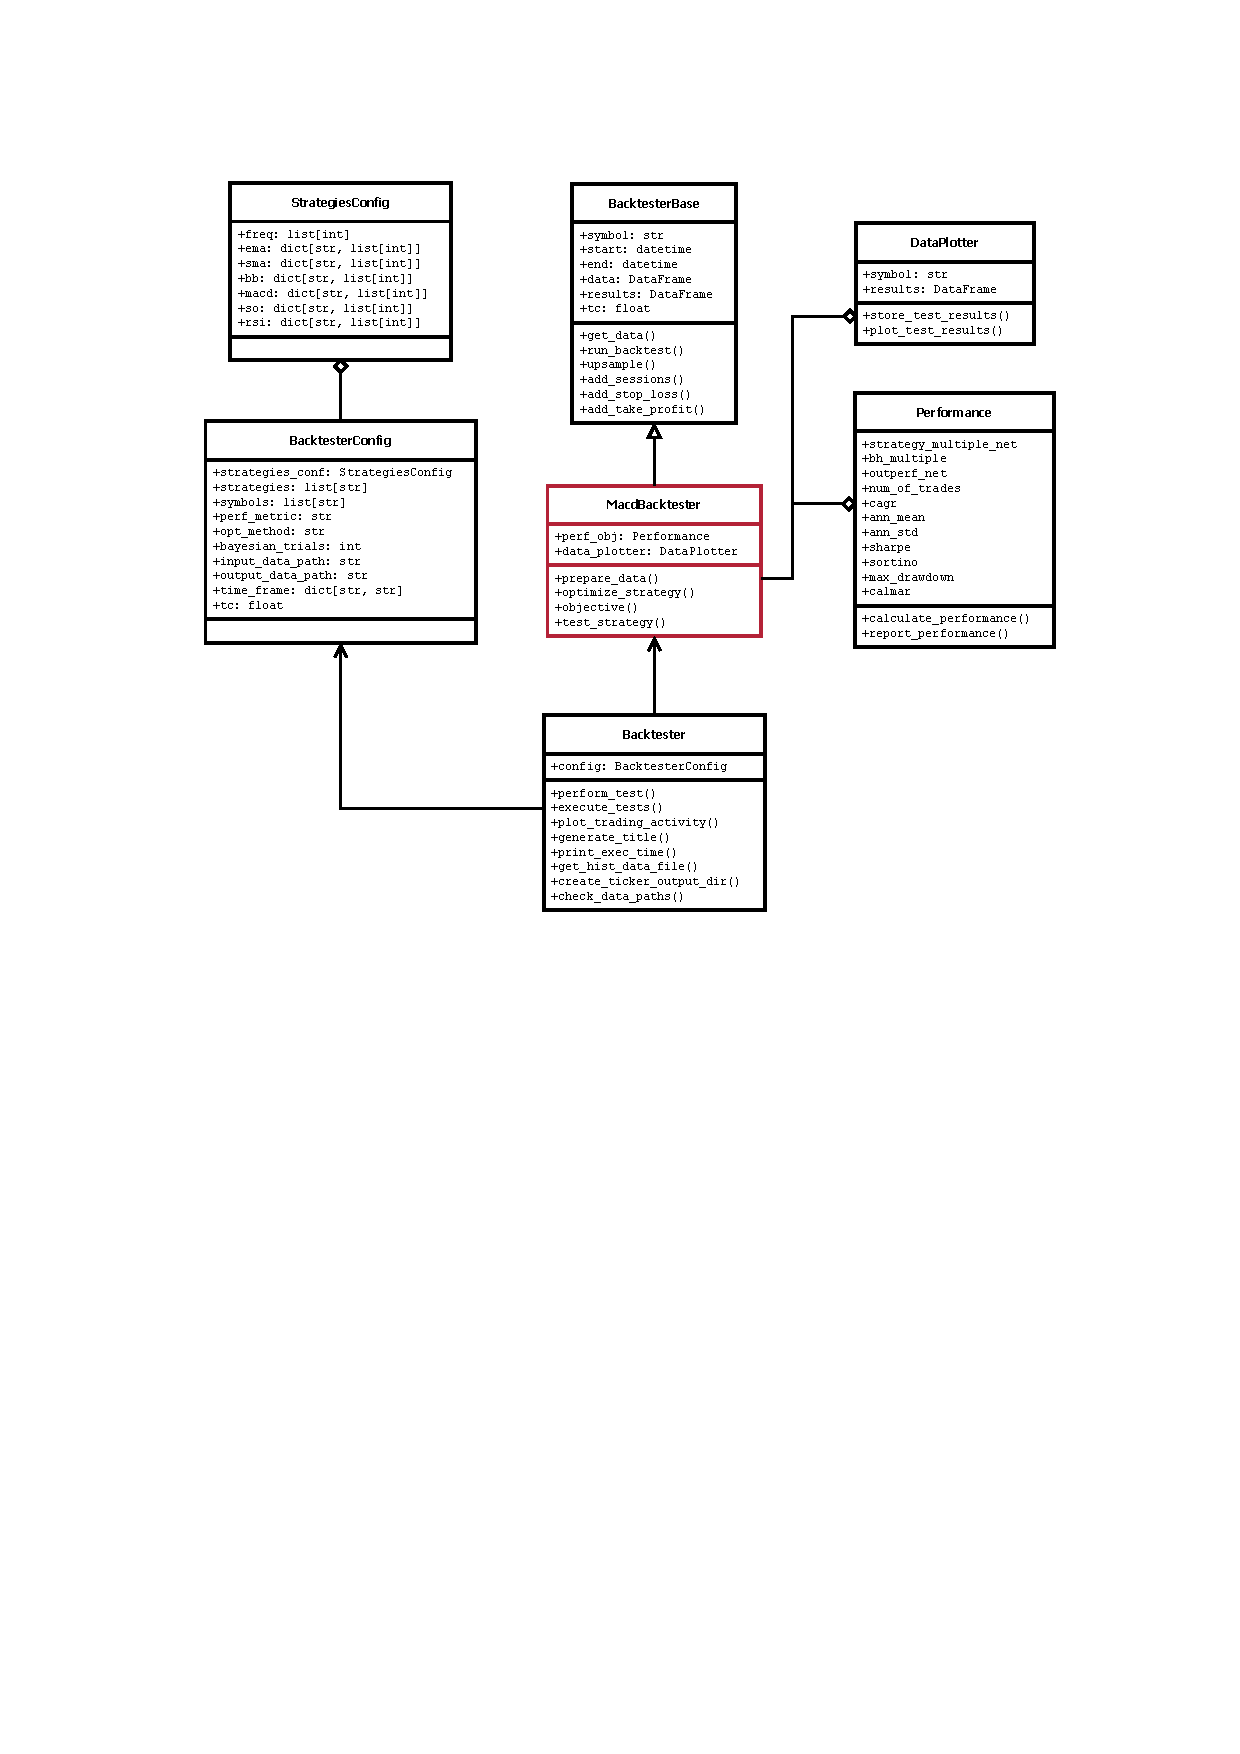
\includegraphics[page=1, trim=30mm 135mm 0 25mm, width=1.1\textwidth, clip]{./uml/backtester_uml.pdf}
\caption{Technical indicator based backtesting architecture.}
\label{fig:tech_indicator_arch}
\end{figure}

\noindent
Technical indicators are mathematical calculations based on historical price, volume, or open interest information that aim to predict future price movements.
Commonly used in technical analysis, these indicators provide insight into the market's direction, strength, momentum, and volatility.